\section*{Triángulo de Pascal}

En las matemáticas, el triángulo de Pascal es una representación de los
coeficientes binomiales ordenados en forma de triángulo. Es llamado así en honor
al filósofo y matemático francés Blaise Pascal, quien introdujo esta notación en
1654, en su Tratado del triángulo aritmético.

\newcommand{\pasc}[2]{
	\pgfkeys{/pgf/fpu}
	\pgfmathparse{round(#1!/((#1-#2)!*#2!))}
	\pgfmathfloattoint{\pgfmathresult}
	\pgfmathresult
}

\begin{figure}[h]
	\centering
	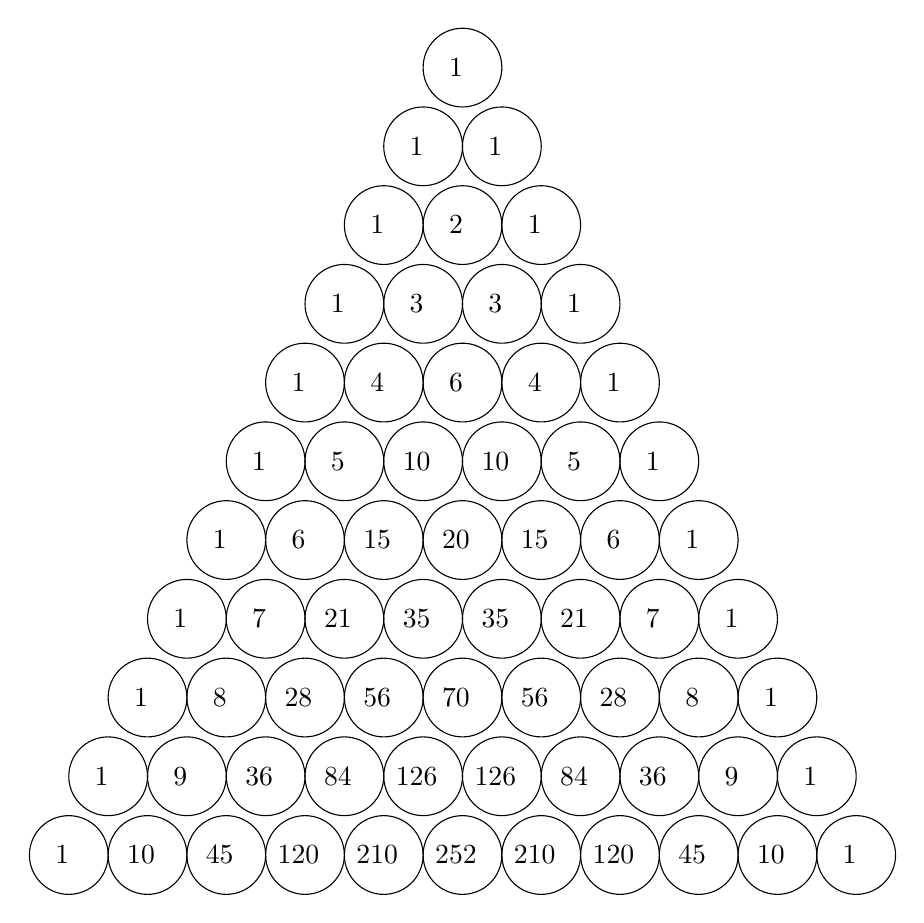
\begin{tikzpicture}
	\pgfmathsetmacro{\N}{10};
	\foreach \i in {0,...,\N}{
		\foreach \j in {0,...,\i}{
			%\pgfmathtruncatemacro{\var}{\pasc{\i}{\j}}
			\node at ({-0.5*\i+\j-0.2},-\i){\pasc{\i}{\j}};
			
			%\ifthenelse{\pasc{\i}{\j}=}{then clause}{else clause}
			% \draw ({-0.5*\i+\j-0.5},-\i+0.5) rectangle
			% ({-0.5*\i+\j-0.5},-\i-0.5);
			\draw ({-0.5*\i+\j},-\i) circle (0.5);
		}
	}
	\end{tikzpicture}
	\caption{Triángulo de Pascal para n=10}
	%\label{pascalTriangle}
\end{figure}

Este triángulo fue ideado para desarrollar las potencias de binomios.

La fórmula del binomio de Newton desarrolla los coeficientes de cada fila en el
triángulo de Pascal. Es por esto que existe una estrecha relación entre el
triángulo de Pascal y el binomios de Newton.

